\part{Théories de la Décision}
\pagebreak

\chapter{Théorie de la décision}

La problématique est celle d'un agent qui doit prendre la meilleure décision, parmi un ensemble de choix possibles (actes), qui selon l'état du monde, mèneront à des conséquences (résultats/outcomes) différentes.\\
\\
Soient A = \{$a_1$, $...$, $a_k$ \} les actes possibles\\
Soient S = \{$s_1$, $...$, $s_m$ \} les états du mondes\\
Soient C = \{$c_1$, $...$, $c_n$ \} les conséquences\\
On n'a donc $A $ x $ S \rightarrow C$\\
Le but est de trouver le $a_i$ qui permet d'obtenir les meilleurs conséquences $c_j$.\\
\\
On distingue 3 type de théories de la décision:
\begin{description}
\item[Décisions sous certitude] il n'y a qu'une état du monde.
\item[Décision dans l'incertain] il y a plusieurs états du monde.
\item[Décision dans le risque] il y a plusieurs états du monde, dont on connait la probabilité.
\end{description}

\pagebreak

\begin{center}
$\begin{tabular}{c|c}
train & voiture\\
\hline
10 & 20 \\
\end{tabular}$
\end{center}
\begin{center}
Décision sous certitude
\end{center}
\vspace{1.5cm}
\begin{center}
$\begin{tabular}{c|cc}
\  & train & voiture\\
\hline
Normal & 10 & 20\\
Bouchon & 10 & 0 \\
\end{tabular}$
\end{center}
\begin{center}
Décision dans incertitude
\end{center}
\vspace{1.5cm}
\begin{center}
$\begin{tabular}{c|c|cc}
\  & \  & train & voiture\\
\hline
Normal & 80\% & 10 & 20\\
Bouchon & 20\% & 10 & 0 \\
\end{tabular}$
\end{center}
\begin{center}
Décision dans le risque
\end{center}

\pagebreak
\section{Décision dans l'incertain}

\subsection{Critère de Laplace}
\begin{description}
\item[] Choisir l'acte dont la conséquence moyenne est la meilleure.
\item[] $argmax_{a \in A}$ $\sum_{s \in S} \frac{1}{|A|} * u(a(s))$
\end{description}

\subsection{Critère de Wald}
\begin{description}
\item[] Choisir l'acte dont la pire conséquence est la meilleure (maximum).
\item[] $argmax_{a \in A}$ $min_{s \in S}$ $u(a(s))$
\end{description}

\subsection{Critère d'Hurwicz}
\begin{description}
\item[] Meilleur compromis entre meilleure et pire conséquences ($a \in [0,1]$)
\item[] $argmax_{a \in A}$ $( \alpha * min_{s \in S}$ $u(a(s))) + (( 1 - \alpha ) * u(a(s)))$
\end{description}

\subsection{Min Max Regret}
\begin{description}
\item[] Choisir l'acte dont on regrettera le moins les conséquences
\item[] $argmax_{a \in A}$ $max_{s \in S}$ $R(a,s)$ avec $R(a,s) = max_{b \in A} u(b(s)) - u(a(s))$
\end{description}

\subsection{Example}

\begin{tabular}{c|ccc|cccc}
\hline
Actes & Etats & du & monde & $ $ & $ $ & $ $ & $ $\\
\hline
$ $  & $s_1$ & $s_2$ & $s_3$ & $Laplace$ & $Wald$ & $Hurwicz_{.5}$ & $MinMax Regret$ \\
\hline
$a_1$ & $55_{21}$ & $10_{12}$ & $13_{13}$ & $26$ & $10$ & $34$ & $\crouge{21}$\\
$a_2$ & $40_{36}$ & $19_3$ & $22_4$ & $\crouge{27}$ & $19$ & $31$ & $36$\\
$a_3$ & $30_{48}$ & $20_0$ & $26_0$ & $26$ & $\crouge{22}$ & $28$ & $46$\\
$a_4$ & $76_0$ & $2_{20}$ & $0_{26}$ & $26$ & $0$ & $\crouge{38}$ & $26$\\
\hline
\end{tabular}

\pagebreak

\subsection{Différents cadres d'incertitude}
\begin{description}
\item[Décision dans le risque (incertitude probabiliste)]: MinMax Regret
\item[Décision dans l'incertain (incertitude qualitative)]: Prade
\item[Décision sous incertitude stricte]: Wald, Hurwicz
\item[Décision sous ignorance total]: Konieczny, Marquis
\end{description}

\pagebreak
\chapter{Théorie des jeux}
\pagebreak

\section{Jeux sous forme stratégique}

Un jeu sous forme stratégique est défini par:
\begin{description}
\item[] un ensemble $N$ = $\{1,....,n\}$ de joueurs
\item[] pour chaque joueurs $i$ un ensemble de stratégies $S_i$ = $\{s_1,.....,S_{n_i}\}$
\item[] pour chaque joueurs $i$ une fonction de valuation $u_i : S_1$ x ... x $S_n \rightarrow R_i$ qui pour un ensemble de stratégies associe les gains du joueur $i$
\end{description}

On notera:\\
\begin{description}
\item[$s$] un profil de stratégies $\{s_1,...,s_n\}$ où $\forall i s_i \in S_i$
\item[$s_{-i}$] le profil $s$ des stratégies autre que celle du joueurs $i$
\item[$S$] l'espace des stratégies 
\end{description}

\subsection{utilité}
On appelle utilité la mesure de chaque situation aux yeux de l'agent, celle ci n'est si une mesure du gain matériel, monétaire, etc, mais une mesure subjective du contentement de l'agent.
\pagebreak
\subsection{jeux sous forme extensive et stratégique}

\begin{center}
\begin{tabular}{c|cc}
$ $ & u & v\\
\hline
x & 4,2 & 3,1\\
y & 2,5 & 9,0\\
\end{tabular}
\end{center}
\begin{center}
Forme stratégique
\end{center}
\ \\
x et y étant les choix représenté par le joueur 1.\\
u et v étant les choix représenté par le joueur 2.\\
Si le joueur 1 choisis x et le joueur 2 v alors le joueur 1 gagnera 3 et le joueur 2 gagnera 1.\\

\begin{center}
\begin{tikzpicture}[->,>=stealth',shorten >=1pt,auto,node distance=3cm,
                    semithick]
  \tikzstyle{every state}=[fill=white,draw=none,text=black]

  \node[state]         (A)                    {$A$};
  \node[state]         (B) [below left of=A]  {$B$};
  \node[state]         (C) [below right of=A] {$C$};
  \node[state]         (XU)[below left of=B]  {$(4,2)$};
  \node[state]         (XV) [below of=B]      {$(3,1)$};
  \node[state]		   (YU) [below of=C]      {$(2,5)$};
  \node[state]    	   (YV)[below right of=C] {$(9,0)$};

  \path (A) edge 			  node {x} (B)
  			edge			  node {y} (C)
  		(B) edge 			  node {u} (XU)
  		    edge 			  node {v} (XV)
  		(C) edge 			  node {u} (YU)
  		    edge			  node {v} (YV);
\end{tikzpicture}
\end{center}
\begin{center}
Forme Extensive
\end{center}

\pagebreak
\subsection{Élimination de stratégies dominées}

Une stratégie $s_i$ est (strictement) dominé pour le joueur $i$ si il existe une stratégie $s_i'$ telle que pour tout profil $s_{-i}$ 
\begin{description}
\item[] $u_i(s_i', s_{-i}) > u_i ( s_i, s_{-i})$
\end{description}

Une stratégie faiblement dominé est sous la forme:
\begin{description}
\item[] $u_i(s_i', s_{-i}) \geq u_i ( s_i, s_{-i})$
\end{description}

\begin{multicols}{3}
[]
\begin{tabular}{c|cc}
$ $ & u & v\\
\hline
x & 4,2 & 3,1\\
y & 2,5 & 9,0\\
\end{tabular}

\begin{tabular}{c|cc}
$ $ & u & $\crouge{v}$\\
\hline
x & 4,2 & $\crouge{3,1}$\\
y & 2,5 & $\crouge{9,0}$\\
\end{tabular}

\begin{tabular}{c|cc}
$ $ & u & $\crouge{v}$\\
\hline
x & 4,2 & $\crouge{3,1}$\\
$\crouge{y}$ & $\crouge{2,5}$ & $\crouge{9,0}$\\
\end{tabular}
\end{multicols}

Le profil (4,2) est sélectionné donc Joueur 1 gagnera 4 et Joueur 2 gagnera 2.\\

\subsection{Équilibre de Nash}

Un jeu peut avoir plusieurs ou aucun équilibre de Nash.\\
\begin{tabular}{c|ccc}
$ $ & u & v & w\\
\hline
x & 3,0 & 0,2 & 0,3\\
y & 2,0 & $\crouge{1,1}$ & 2,0\\
z & 0,3 & 0,2 & 3,0\\
\hline
\end{tabular}
\ \\\\
Deux équilibre de Nash sont interchangeable si la permutation des termes gauche garde l'équilibre de Nash actif.\\

Voici un cas particulier:
\begin{tabular}{c|cc}
$ $ & u & v\\
\hline
x & 2,1 & 0,0\\
y & 0,0 & 1,2\\
\end{tabular}

Deux équilibre de Nash sont présent $\crouge{(2,1)}$ et $\crouge{(1,2)}$.
Comme il y a une hésitation entre les deux cas, alors l'utilisation du flip coin est envisageable:
\begin{description}
\item[] $u_1(<(x, 1/2), (y, 1/2)>) = 1/2 * 2 + 1/2 * 0 = 1$
\item[] $u_1(<(u, 1/2), (v, 1/2)>) = 1/2 * 0 + 1/2 * 1 = 1/2$
\end{description}

\subsection{Critère de Pareto}

\begin{multicols}{2}
[Soit la table:]

\begin{tabular}{c|cc}
$ $ & u & v\\
\hline
x & 4,4 & 3,1\\
y & 2,3 & 7,5\\
\end{tabular}
\vspace{1.5cm}

\begin{description}
\item[] Pour u, x est meilleur que y
\item[] Pour v, y est meilleur que x
\item[] Pour x, u est meilleur que v
\item[] Pour y, v est meilleur que u
\end{description}

\end{multicols}

\begin{multicols}{2}
[Un profil s domine un profil s' dans le sens de Pareto si pour tout les joueurs s est au moins meilleur que s' et que pour un joueur s est meilleur strictement que s'.\\
Un profil s domine strictement un profil s' dans le sens de Pareto si pour tout les joueurs s est meilleur que s'.\\
]

\begin{tabular}{c|cc}
$ $ & u & v\\
\hline
x & 4,4 & $\crouge{3,1}$\\
y & $\crouge{2,3}$ & 7,5\\
\end{tabular}

\begin{description}
\item[] (x,u) 4,4
\item[] (y,v) 7,5 est meilleur
\end{description}

\end{multicols}

\subsection{Niveau de sécurité}
Pour un tableau:

\begin{tabular}{c|cc}
$ $ & u & v\\
\hline
x & 9,9 & 0,8\\
y & 8,0 & 7,7\\
\end{tabular}
\ \\\\
Dans le cas d'un jeu avec des joueurs non rationnel, l'un des deux joueur peut duper l'autre et ainsi gagner 8 et faire gagner 0 à l'autre joueur. \\\\
On défini le niveau de sécurité d'une stratégie $s_i$ pour le joueur i comme le gain minimum que peut apporter cette stratégie quel que soit le choix des autres joueurs.\\
On défini le niveau de sécurité d'un joueur i comme le niveau de sécurité maximal des stratégies de i.\\

Le meilleur choix serait de prendre (y,v) pour assurer un minimum de gain pour chaque personnes.\\

\subsection{autres Stratégies}
Jusque la nous avons utilisé que les stratégies pures, c'est à dire les option qui se présente au joueurs.\\
Une stratégies mixte est une distribution de probabilité sur l'ensemble des stratégies pures.\\
Une stratégie local du joueur $i$ est une distribution de probabilités $p_i$ définit sur l'ensemble des stratégies pure du joueurs $i$.\\
Une stratégie comportemental du joueur $i$ est un vecteur de stratégies locales du joueur $i$.\\

\subsection{Équilibre de Nash en stratèges mixtes}
Soit le problème:
\begin{tabular}{cc|cc}
$ $ &$ $ & y & 1-y\\
\hline
$ $& $ $ & f & c\\
\hline
x & f & 2,1 & 0,0\\
1-x & c & 0,0 & 1,2\\
\end{tabular}

Soit y, la probabilité avec laquelle le joueur 2 jour f, quelle est la meilleure réponse du joueur 1?:
\begin{description}
\item[] $u_1(<(f, y), (c, 1-y)>) = y*2 + (1-y)*0 = 2y$
\item[] $u_1(<(f, y), (c, 1-y)>) = y*0 + (1-y)*1 = 1-y$
\end{description}

Donc:
\begin{description}
\item[] Si $2y > 1 - y$ avec ($y > 1/3$), la meilleur réponse du joueur 1 est de jouer $f$
\item[] Si $2y < 1 - y$ avec ($y < 1/3$), la meilleur réponse du joueur 1 est de jouer $c$
\item[] Si $2y = 1 - y$ avec ($y = 1/3$), le joueur 1 peut jouer l'un ou l'autre.
\end{description}

Soit x, la probabilité avec laquelle le joueur 1 jour f, quelle est la meilleure réponse du joueur 2?:
\begin{description}
\item[] $u_1(<(f, x), (c, 1-x)>) = x*1+(1-x)*0 = x$
\item[] $u_1(<(f, x), (c, 1-x)>) = x*1+(1-x)*0 = 2(1-x)$
\end{description}

Donc:
\begin{description}
\item[] Si $x > 2(1-x)$ avec ($x > 2/3$), la meilleur réponse du joueur 2 est de jouer $f$
\item[] Si $x < 2(1-x)$ avec ($x < 2/3$), la meilleur réponse du joueur 2 est de jouer $c$
\item[] Si $x = 2(1-x)$ avec ($x = 2/3$), le joueur 2 peut jouer l'un ou l'autre.
\end{description}


\subsection{Représentation graphique du jeu}
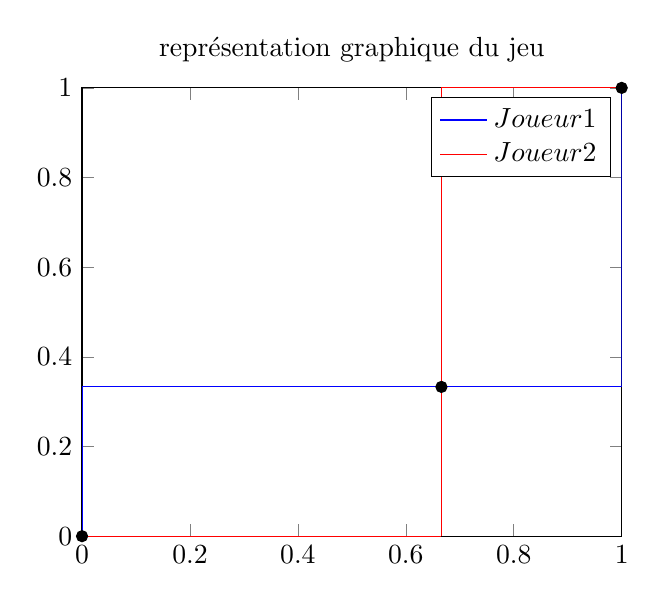
\begin{tikzpicture}
\begin{axis}[
	xmin=0, xmax=1, ymin=0, ymax=1, title={représentation graphique du jeu}
	]
    \addplot [color=blue] coordinates { (0,0)(0,0.333) };
    \addplot [color=red] coordinates { (0,0)(0.666,0) };
    \addplot [color=blue] coordinates { (0,0.333)(1,0.333) };
    \addplot [color=blue] coordinates { (1,0.333)(1,1) };
    \addlegendentry{$Joueur 1$}
    \addplot [color=red] coordinates { (0.666,0)(0.666,1) };
    \addplot [color=red] coordinates { (0.666,1)(1,1) };
    \addlegendentry{$Joueur 2$}
    \addplot [only marks, mark=*, color=black] coordinates { (0,0) (1,1) (0.666,0.333) };
\end{axis}
\end{tikzpicture}

\pagebreak
\subsection{Coopération}

\begin{tabular}{c|cc}
$ $ & f & c\\
\hline
f & 2,1 & 0,0\\
c & 0,0 & 1,2\\
\end{tabular}

Que se passe t'il si les 2 joueurs peuvent communiquer avant de jouer?:
\formula{$u_1 = u_2 = \frac{1}{2} * 2 + \frac{1}{2} = \frac{3}{2}$}

Lorsque tout les joueurs peuvent observer un même événement aléatoire, ils peuvent alors s'accorder sur des équilibres corrélés.\\
Selon un accord prit via un flip coin, ou via une parution d'un évènement, si les deux joueurs se mette d'accord sur le fait de tirer $f$ ou $c$, mais le joueur désavantagé peut ne pas jouer le choix prit, mais il s'expose à ne rien gagner.\\

\subsection{Itération le dilemme des prisonniers}
Deux personne sont arrêtées ensemble en possession d'armes à feu sont soupçonnés d'un délit fait en commun, Les policiers les séparent et disent à chacun:
\begin{description}
\item[] Si l'un des deux avoue et que l'autre ne dit rien, le premier est libéré et le second emprisonné 5 ans.
\item[] Si les deux avouent, les deux iront 4 ans en prison.
\item[] Si les deux ne disent rien alors ils seront emprisonné 2 ans.
\end{description}

Donnant le tableau suivant:
\begin{tabular}{c|cc}
$ $ & P2 avoue & P2 rien\\
\hline
P1 avoue & 4,4 & 0,5\\
P1 rien  & 5,0 & 2,2\\
\end{tabular}

\ \\
Mais les valeurs inscrit ne représente pas le gain, donc il faut inverser les valeurs par rapport au maximum ($5$):\\

\begin{tabular}{c|cc}
$ $ & P2 avoue & P2 rien\\
\hline
P1 avoue & 1,1 & 5,0\\
P1 rien  & 0,5 & 3,3\\
\end{tabular}

Si le joueur 1 avoue et le joueur 2 ne dit rien alors le joueur 1 gagnera 5 ans et le joueur 2 gagner 0 ans (car il sera en prison).\\

\subsection{DIP Itérations}

\begin{description}
\item[] Les joueurs se rencontrent plusieurs fois
\item[] A chaque itération les joueurs ont connaissances des coups précédents 
\item[] ils ne connaissent pas les terme du jeu
\item[] le gain d'un joueur est le cumul des gains de chaque rencontre
\item[] Pour favoriser le coopération on ajoute la contrainte \formula{$X + T < 2R$}
\end{description}
\scalebox{0.8}{
\begin{tabular}{c|cc}
$ $ & Coopérer & non coopérer\\
\hline
Coopérer & $R=3$ récompense pour coopération mutuelle & $S=0$ salaire de la dupe\\
non coopérer & $T=5$ tentation à trahir & $P=1$ punition pour la trahison mutuelle\\
\end{tabular}}

\subsection{Les Stratégies}

Dans une rencontre les joueurs peuvent avoir plusieurs comportements diffèrent, appliquons les sur le problème DIP:
\begin{description}
\item[gentille] le joueur sera gentil quitte à perdre
\item[méchante] le joueur ne laisse rien passé, tout doit être acquérir 
\item[par pattern] suivre la même séquence de choix à l'infini
\item[rancunière] donnant donnant jusqu'à l'erreur de l'adversaire
\item[lunatique] aléatoirement
\item[majoritaire gentille] joue ce que l'autre joue
\item[majoritaire méchante] trahir
\item[donnant donnant] joue le coup précédent de l'autre
\end{description}

Quand on fait jouer ses stratégies dans le cadre d'un tournois on obtient les scores suivant:

\begin{center}
\begin{tabular}{c|cc}
place & stratégie & points \\
\hline
1 & donnant donnant & 42 \\
2 & majoritaire gentille & 19 \\
3 & rancunière & 4\\
4 & lunatique  & 0\\
\end{tabular}
\end{center}
\ \\
le top 3 n'est pas compliqué à déduire, se sont tous des stratégies adaptatif (qui s'adapte à l'adversaire).\\
le top 2 a un pouvoir pour pardonner l'adversaire donc un jugement moins punitif.\\
le top 1 est simple, il incarne la simplicité.\\
la gentillesse prime aussi.\\

\pagebreak
\section{Jeux répété}

Soit un jeu $G = \{S, \{u_i \} i=1,...n \}$ où $S$ est l'ensemble fini des profils stratégie et $u_i$ est la fonction d'utilité du joueur $i$.\\
On note $(G,T)$ le jeu répété obtenu en jouant $T$ fois le jeu de base $G$, $(G,\infty)$ correspond à un nombre infini de tour.\\

On peut également distinguer les jeux répété un nombre fini, mais indéfini de fois : à chaque tour, il y a une probabilité $1 - q$ 
que le jeu s'arrête.\\
Facteur d'actualisation: Lorsqu'un jeu est répété, il se peut que les gains obtenus à l'itération courante $u_t$ soient plus/moins importants aux yeux de l'agent que les gains  l'itération suivante $u_{t+1}$. Pour modéliser cela on peut utiliser un facteur d'actualisation $\phi$:
\formula{$u_t = \phi u_{t+1}$}

Le facteur d'actualisation $\phi = \frac{u_t}{u_{t+1}}$ représente donc l'attrait du joueur pour les gains actuels.

\subsection{Jeux à deux joueurs à somme nulle}

Dans le cas d'un jeu à somme nulle pour chaque case le joueur 1 va gagner la somme indiqué et le joueur 2 va perdre la somme indiqué:\\
\begin{center}
\begin{tabular}{c|cccc}
$ $ & $y_1$ & $y_2$ & $y_3$ & $y_4$ \\
\hline
$x_1$ & 18 & 3 & 0 & 2\\
$x_2$ & 0 & 3 & 8 & 20\\
$x_3$ & 5 & 4 & 5 & 5\\
$x_4$ & 9 & 3 & 0 & 20\\
\end{tabular}
\end{center}
\ \\
si le joueur 1 prend $x_1$ et le joueur 2 $y_1$ alors le joueur 1 gagnera 18 et le joueur 2 perdra 18.\\

Le joueur 1 tente de maximiser son niveau de sécurité:
\formula{$v_x = max_i(min_j u(x_i,y_j))$}

Le joueur 2 tente de minimiser le niveau de sécurité du joueur 1:
\formula{$v_y = min_j(max_i u(x_i,y_j))$}

\subsection{Jeu sous forme extensive}

Un jeu se déroulant de la racine jusqu'à une feuille, le noeud indique quel joueur doit jouer, donc un ordre de passage est explicite.\\

Soit le jeu suivant sous forme d'arbre:

\begin{center}
\scalebox{0.8}{
\begin{tikzpicture}[->,>=stealth',shorten >=1pt,auto,node distance=3cm,
                    semithick]
  \tikzstyle{every state}=[fill=white,draw=none,text=black]

  \node[initial, state](A)                    {$1$};
  \node[state]         (B) [below of=A]       {$2$};
  \node[state]         (C) [right of=A]       {$3$};
  \node[state]		   (D) [right of=C]       {$(3,2,2)$};
  \node[state]         (AA)[below left of=A]  {$(3,0,0)$};
  \node[state]         (BA)[below left of=B]  {$(4,2,4)$};
  \node[state]		   (BB)[below right of=B] {$(2,3,1)$};
  \node[state]    	   (CA)[below  of=C]      {$(1,0,3)$};

  \path (A) edge 			  node {x} (AA)
  			edge			  node {y} (B)
  		    edge 			  node {z} (C)
  		(B) edge 			  node {w'} (BA)
  		    edge 			  node {u'} (BB)
  		(C) edge              node {u}  (CA)
  		    edge 			  node {w}  (D);
\end{tikzpicture}
}\end{center}

\begin{multicols}{2}
[Via la récurrence à rebours, On remonte les noeuds optimaux de l'arbre vers la racine:]
\scalebox{0.7}{
\begin{tikzpicture}[->,>=stealth',shorten >=1pt,auto,node distance=3cm,semithick]
  \tikzstyle{every state}=[fill=white,draw=none,text=black]

  \node[initial, state](A)                    {$1$};
  \node[state]         (B) [below of=A]       {$(2,3,1)$};
  \node[state]         (C) [right of=A]       {$(1,0,3)$};
  \node[state]         (AA)[below left of=A]  {$(3,0,0)$};

  \path (A) edge 			  node {x} (AA)
  			edge			  node {y} (B)
  		    edge 			  node {z} (C);
\end{tikzpicture}
}
\scalebox{0.7}{
\begin{tikzpicture}[->,>=stealth',shorten >=1pt,auto,node distance=3cm,semithick]
  \tikzstyle{every state}=[fill=white,draw=none,text=black]

  \node[initial, state](A)                    {$(3,0,0)$};

\end{tikzpicture}
}
\end{multicols}

\subsection{sous jeu}
Un sous jeu d'un jeu sous forme extensive est un jeu composé d'un noeud (qui est un ensemble d'information singleton) de tous les noeuds successeurs de ce noeud, de tout les arcs reliant ces noeuds, et des unités associées à tout les noueds terminaux successeurs.
\\
Le grand arbre ci dessus contient 3 sous jeux ayant comme racine (1,2,3).\\

\pagebreak
\subsection{Menaces non crédibles}

\begin{multicols}{2}
[Voici le même jeu sous forme de tableau et sous forme d'arbre]
\scalebox{0.65}{
\begin{tikzpicture}[->,>=stealth',shorten >=1pt,auto,node distance=3cm,semithick]
  \tikzstyle{every state}=[fill=white,draw=none,text=black]

  \node[initial, state](A)                    {$1$};
  \node[state]         (B) [below of=A]       {$2$};
  \node[state]         (AA)[below left of=A]  {$(2,2)$};
  \node[state]         (BA)[below left of=B]  {$\crouge{(3,1)}$};
  \node[state]		   (BB)[below right of=B] {$(0,0)$};

  \path (A) edge 			  node {x} (AA)
  			edge			  node {y} (B)
  		(B) edge 			  node {u} (BA)
  		    edge 			  node {v} (BB);
\end{tikzpicture}
}

\begin{tabular}{c|cc}
$ $ & u & v\\
\hline
x & (2,2) & $\crouge{(2,2)}$\\
y & $\crouge{(3,1)}$ & (0,0)\\
\end{tabular}
\end{multicols}

L'équilibre de Nash de l'arbre indique que la meilleur stratégie (d'un point de vue rationnel) est $(3,1)$ et via le tableau on obtient $\{(3,1),(2,2)\}$.\\
l'équilibre de Nash $(xv)$ n'est pas crédible car il repose sur la menace non-crédible du joueur 2 de joueur $v$, autrement dit, dans le premier tour, si le joueur 1 joue $x$, le joueur 2 n'a aucun choix à faire, hors dans le tableau le joueur 2 peut proposer un choix.\\

Un équilibre de Nash d'un jeu sous forme extensive est un équilibre parfait en sous jeu si toute restriction du profil de stratégies à un sous jeu est un équilibre de Nash pour ce sous jeu.\\
Pour les jeux à informations parfaites, la notion d'équilibre parfait en sous jeu coïncide avec la notion de récurrence à rebours.\\ 

\pagebreak
\subsection{Promesse non crédible}
Soit un contrat pour travailler en entreprise, le joueur 2 étant vous et le joueur 1 étant l'entreprise:

\begin{center}
\scalebox{0.7}{
\begin{tikzpicture}[->,>=stealth',shorten >=1pt,auto,node distance=3cm,semithick]
  \tikzstyle{every state}=[fill=white,draw=none,text=black]

  \node[initial, state](A)                    {$2$};
  \node[state]         (B) [below right of=A] {$1$};
  \node[state]         (AA)[below left of=A]  {$\crouge{(0,0)}$};
  \node[state]         (BA)[below left of=B]  {$(2,-1)$};
  \node[state]		   (BB)[below right of=B] {$(1,1)$};

  \path (A) edge 			  node {décliner} (AA)
  			edge			  node {accepter} (B)
  		(B) edge 			  node {Exploiter} (BA)
  		    edge 			  node {Ne pas exploiter} (BB);
\end{tikzpicture}
}
\end{center}
Dans le cas d'un contrat non répété il est mieux de choisir $\crouge{(0,0)}$, mais dans le cas d'un jeu répété si vous êtes le premier candidat et que vous acceptez le poste mais que vous vous faite exploiter, alors vous aller altérer les nouveaux candidats pour qu'ils choisis l'option de ne pas aller travailler la bas, donc l'entreprise ne devrait pas vous exploiter pour son bien.\\

\subsection{Limite de la récurrence à rebours}

Soit le jeu suivant, vous êtes le joueur 1:
\begin{center}
\scalebox{0.6}{
\begin{tikzpicture}[->,>=stealth',shorten >=1pt,auto,node distance=3cm,semithick]
  \tikzstyle{every state}=[fill=white,draw=none,text=black]

  \node[initial, state](A)                    {$1$};
  \node[state]         (B) [right of=A]       {$2$};
  \node[state]         (C) [right of=B]       {$1$};
  \node[state]         (D) [right of=C]       {$2$};
  \node[state]         (AA)[below of=A]       {$\crouge{(98,98)}$};
  \node[state]         (BA)[below of=B]       {$(97,100)$};
  \node[state]         (CA)[below of=C]       {$(99,99)$};
  \node[state]         (DA)[below of=D]       {$(98,101)$};
  \node[state]         (DB)[right of=D]       {$(100,100)$};
  
  

  \path (A) edge 			  node {D} (AA)
  			edge			  node {R} (B)
  		(B) edge 			  node {D} (BA)
  		    edge 			  node {R} (C)
  		(C) edge              node {D} (CA)
  		    edge              node {R} (D)
  		(D) edge              node {D} (DA)
  		    edge 			  node {R} (DB);
\end{tikzpicture}
}
\end{center}
Le calcule de l'équilibre de Nash nous donne $\crouge{(98,98)}$ mais cette équilibre ne marche que si le joueur 2 est un robot / rationnel, si on indique que les somme sont des Millions d'euro, les choix seront bien plus différent, si les deux joueurs sont altruiste alors les deux vont gagner $(100,100)$ si l'un des joueur est mauvais alors celui ci va aller le plus haut possible et choisir $D$ juste en guise de dernier choix.\\

\pagebreak
\section{Jeux coopératifs à 2 joueurs}

%% fill

\pagebreak